\documentclass[10pt]{beamer}

\newcommand{\lectnum}{L03}
\newcommand{\lecttitle}{Linear Regression and Classification: Part I}

\usepackage{amsmath, amssymb, graphicx}
\usepackage[]{algorithm2e}
\usepackage{pdfpages}
\usepackage{bm}
\usepackage{relsize}
\usepackage[british]{babel}
\usepackage{tikz,tikzsymbols}
\usepackage{hyperref}
\usepackage{cancel}
\usepackage{caption,subcaption}
\usepackage{adjustbox}
\usepackage{overpic}
\usepackage[UKenglish]{isodate}

\usetikzlibrary{arrows,decorations.markings,positioning}

\newcommand{\bs}{\boldsymbol}


\hypersetup{colorlinks,linkcolor=,urlcolor=blue}
\newenvironment{titledslide}[1]{\begin{frame}\frametitle{#1}}{\end{frame}}

\mode<presentation>{\setbeamercovered{transparent}}

\setbeamertemplate{sidebar right}{}
\setbeamertemplate{footline}{%
\leavevmode%
\hbox to \paperwidth{\hfil\usebeamertemplate***{navigation symbols}%
\hspace{0.4cm}\lectnum: \insertframenumber{}/\inserttotalframenumber\hspace*{0.4cm}}%
\vspace{2pt}}

\author{Mengyan Zhang}

\title{COMS20018, Introduction to AI:\\ \vspace{5pt} \lecttitle}

\institute{School of Computer Science\\University of Bristol}
\date{28th September 2026}

%%%%%%%%%%%%%%%%%%%%%%%%%%%%%%%%%%%%%%%%%%%%%%%%%%%%%%%%%%%%%%%%%%%%%%

\begin{document}
%%%%%%%%%%%%%%%%%%%%%%%%%%%%%%%%%%%%%%%%%%%%%%%%%%%%%%%%%%%%%%%%%%%%%%

\begin{frame}[fragile]
  \begin{tikzpicture}[remember picture, overlay]
    \node[anchor=north west, xshift=0.4cm, yshift=-0.4cm] at (current page.north west)
      {
\includegraphics[width=3.4cm]{figures/uob_logo.png}};
  \end{tikzpicture}
  \titlepage
\end{frame}
%%%%%%%%%%%%%%%%%%%%%%%%%%%%%%%%%%%%%%%%%%%%%%%%%%%%%%%%%%%%%%%%%%%%%%
\begin{frame}[fragile]

  \frametitle{Agenda}
  \begin{itemize}
  \item Categories of machine learning \hfill
    \begin{itemize}
    \item Supervised, unsupervised, reinforcement learning
    \item Self-supervised \& semi-supervised learning
    \item Where today fits: regression
    \end{itemize}
  \item Model selection \hfill
    \begin{itemize}
    \item Training, validation \& test data
    \item Cross-validation
    \end{itemize}
  \item Linear regression: least squares \hfill
    \begin{itemize}
    \item Curve fitting
    \item Linear basis function models
    \item Least squares
    \item The normal equations
    \item Worked example
    \item Evaluation metrics
    \end{itemize}
  \end{itemize}

\end{frame}
%%%%%%%%%%%%%%%%%%%%%%%%%%%%%%%%%%%%%%%%%%%%%%%%%%%%%%%%%%%%%%%%%%%%%%
\begin{frame}[fragile]
\frametitle{Categories of machine learning (1/3)}

\centerline{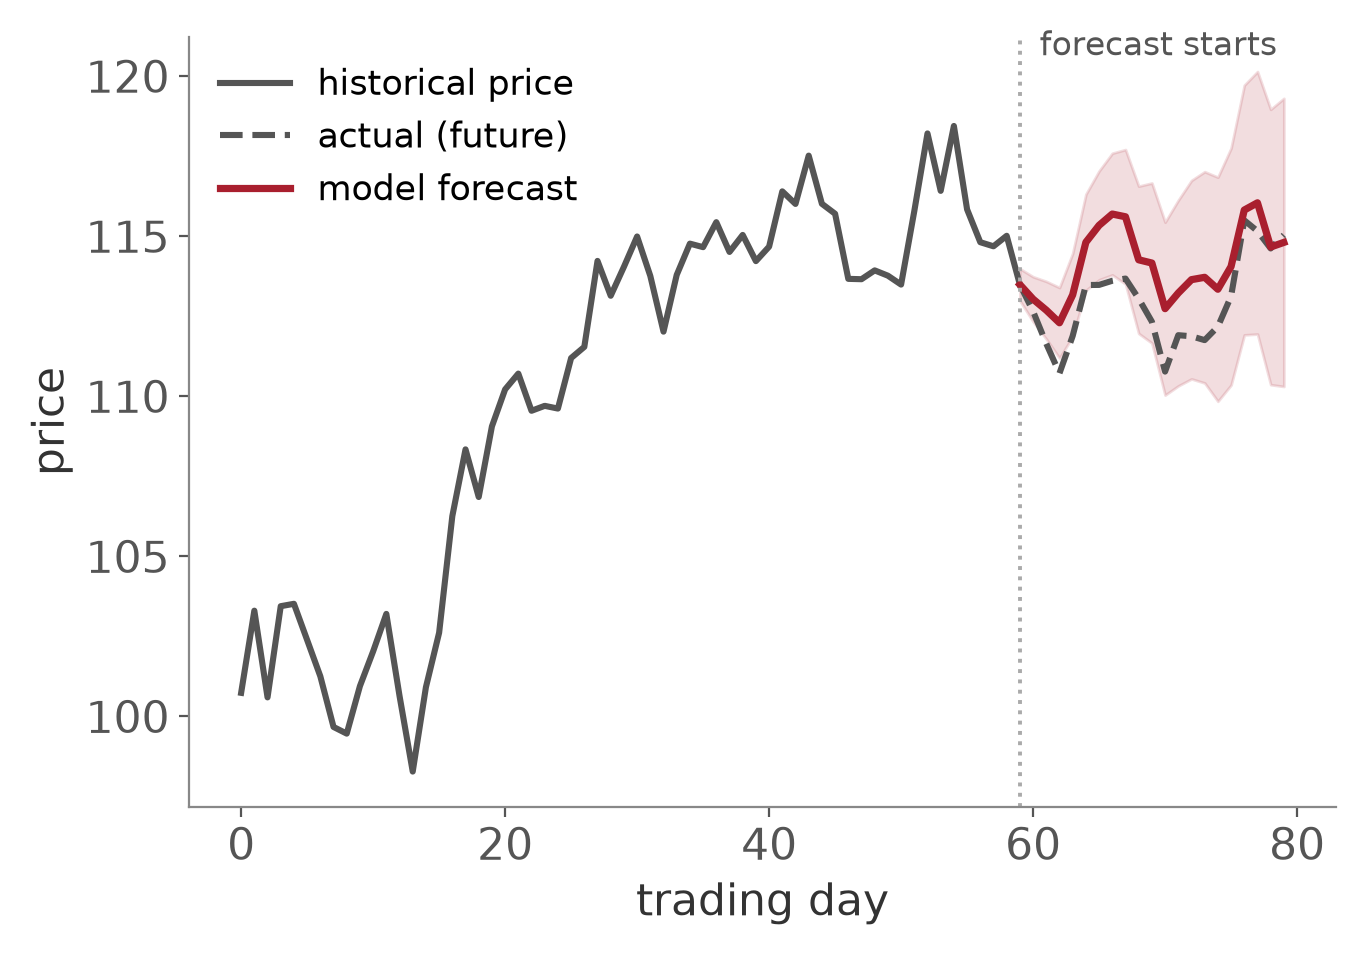
\includegraphics[height=3.6cm]{figures/finance_chart.png}}

\vspace{6pt}
\centerline{\textbf{Supervised Learning}, forecasting a price (regression)}

\vspace{14pt}
\begin{itemize}
\item Given labelled examples $\{(x_n,t_n)\}_{n=1}^N$, learn a mapping
  $x \mapsto t$.
\end{itemize}

\end{frame}
%%%%%%%%%%%%%%%%%%%%%%%%%%%%%%%%%%%%%%%%%%%%%%%%%%%%%%%%%%%%%%%%%%%%%%
\begin{frame}[fragile]
\frametitle{Categories of machine learning (2/3)}

\centerline{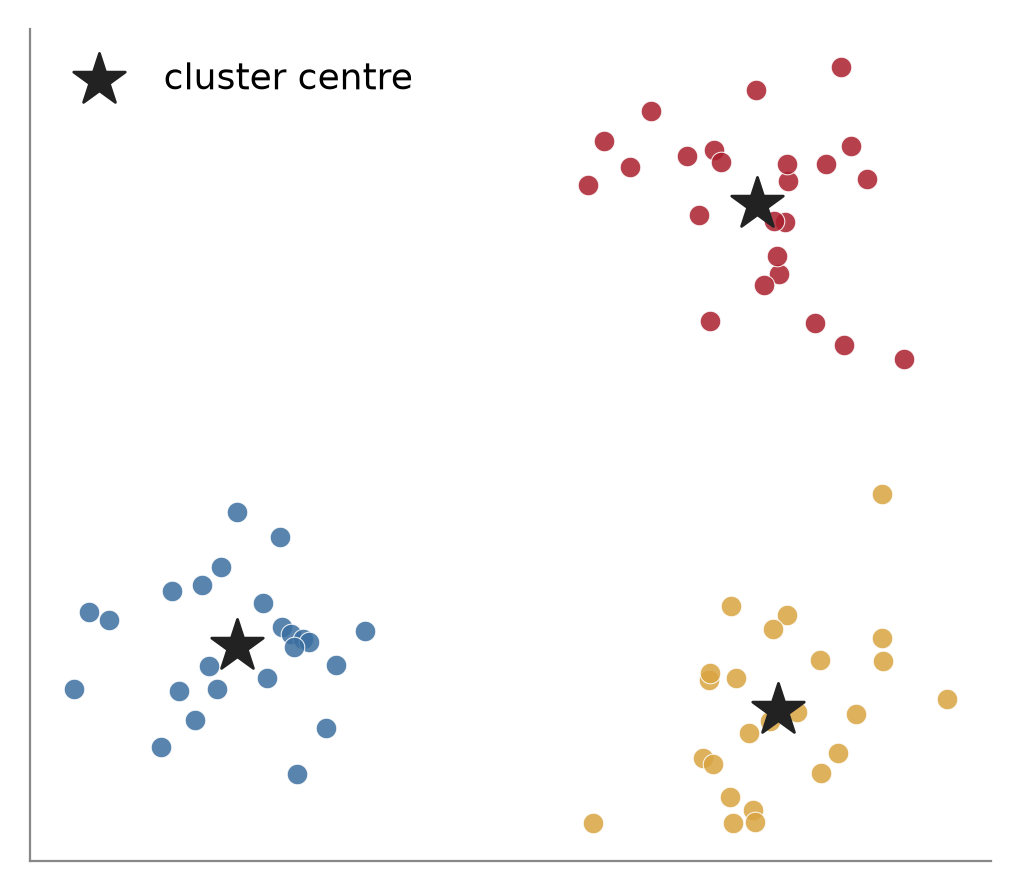
\includegraphics[height=3.6cm]{figures/unsupervised_diagram.png}}

\vspace{6pt}
\centerline{\textbf{Unsupervised Learning}, customer segmentation (clustering)}

\vspace{14pt}
\begin{itemize}
\item Given only \emph{unlabelled} data $\{x_n\}_{n=1}^N$, find structure,
  e.g.\ clusters, or the underlying density. 
\end{itemize}

\end{frame}
%%%%%%%%%%%%%%%%%%%%%%%%%%%%%%%%%%%%%%%%%%%%%%%%%%%%%%%%%%%%%%%%%%%%%%
\begin{frame}[fragile]
\frametitle{Categories of machine learning (3/3)}

\centerline{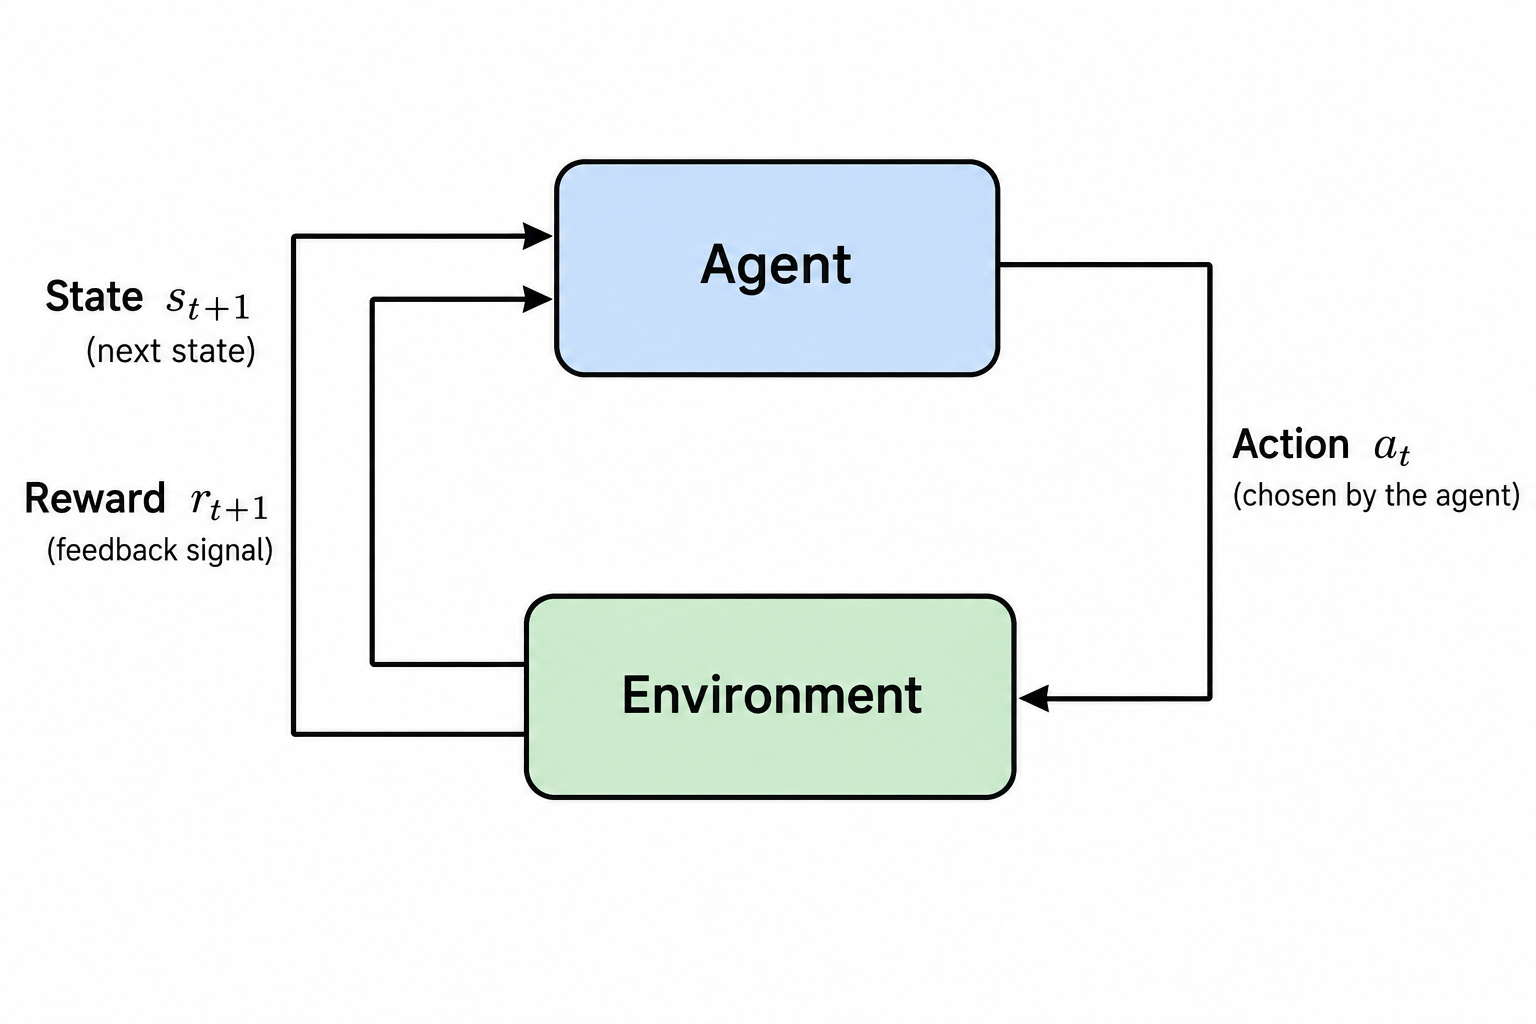
\includegraphics[height=4.2cm]{figures/rl_loop.png}}

\vspace{6pt}
\centerline{\textbf{Reinforcement Learning} -- e.g.\ AlphaGo (game-playing)}

\vspace{10pt}
\begin{itemize}
\item An agent learns from \emph{reward} signals produced by its own
  actions, not from labelled examples; covered by Week 9.
\end{itemize}

\end{frame}
%%%%%%%%%%%%%%%%%%%%%%%%%%%%%%%%%%%%%%%%%%%%%%%%%%%%%%%%%%%%%%%%%%%%%%
\begin{frame}[fragile]
\frametitle{Two more flavours: self-supervised \& semi-supervised}

\begin{columns}[T]
\begin{column}{0.5\textwidth}
\centerline{\textbf{Self-supervised}}
\vspace{4pt}
\centerline{\resizebox{0.98\textwidth}{!}{%
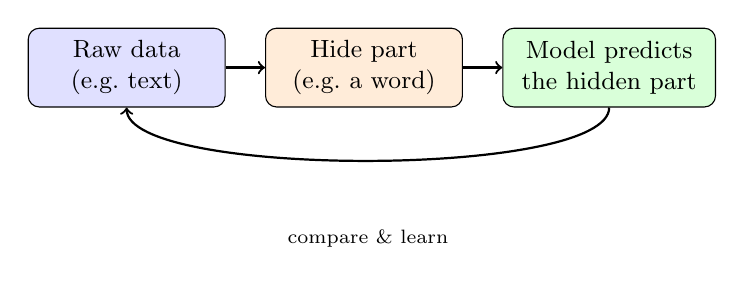
\begin{tikzpicture}[
  box/.style={draw, rounded corners, align=center, font=\small,
    minimum height=1cm}
]
  \node[box, fill=blue!12, minimum width=2.5cm] (raw) {Raw data\\(e.g.\ text)};
  \node[box, fill=orange!15, minimum width=2.5cm, right=0.5cm of raw] (mask)
    {Hide part\\(e.g.\ a word)};
  \node[box, fill=green!15, minimum width=2.7cm, right=0.5cm of mask] (pred)
    {Model predicts\\the hidden part};
  \draw[->, thick] (raw) -- (mask);
  \draw[->, thick] (mask) -- (pred);
  \draw[->, thick] (pred.south) .. controls +(0,-0.9) and +(0,-0.9) .. (raw.south)
    node[midway, below=0.75cm, font=\scriptsize] {compare \& learn};
\end{tikzpicture}}}
\vspace{6pt}
\begin{itemize}
\small
\item Labels generated automatically from the data itself, e.g.\
  predict the next word, or a masked-out image patch
\item Powers modern LLM pretraining; no human-annotated labels needed
\end{itemize}
\end{column}
\begin{column}{0.5\textwidth}
\centerline{\textbf{Semi-supervised}}
\vspace{4pt}
\centerline{\resizebox{0.9\textwidth}{!}{%
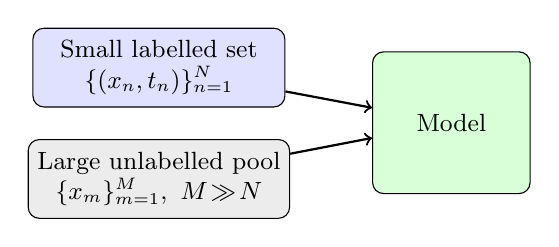
\begin{tikzpicture}[
  box/.style={draw, rounded corners, align=center, font=\small,
    minimum height=1cm}
]
  \node[box, fill=blue!12, minimum width=3.2cm] (lab) {Small labelled set\\$\{(x_n,t_n)\}_{n=1}^N$};
  \node[box, fill=gray!15, minimum width=3.2cm, below=0.4cm of lab] (unlab)
    {Large unlabelled pool\\$\{x_m\}_{m=1}^M,\ M\!\gg\! N$};
  \node[box, fill=green!15, minimum width=2cm, minimum height=1.8cm,
    right=1.1cm of lab, yshift=-0.7cm] (model) {Model};
  \draw[->, thick] (lab) -- (model);
  \draw[->, thick] (unlab) -- (model);
\end{tikzpicture}}}
\vspace{6pt}
\begin{itemize}
\small
\item Labels are expensive, raw data is cheap; use the unlabelled
  data to learn structure, then fit it to the few labels you have
\end{itemize}
\end{column}
\end{columns}

\vspace{6pt}
\begin{itemize}
\item[$\Rightarrow$] Both sit between supervised and unsupervised
  learning, useful whenever labels are scarce but data is not
\end{itemize}

\end{frame}
%%%%%%%%%%%%%%%%%%%%%%%%%%%%%%%%%%%%%%%%%%%%%%%%%%%%%%%%%%%%%%%%%%%%%%
\begin{frame}[fragile]
\frametitle{Model selection: training, validation \& test data}

\begin{itemize}
\item Choosing between candidate models or hyperparameters (e.g.\ the
  polynomial order $M$ we meet next) is a problem for \emph{any}
  learning method, not just parametric ones like ours today.
\item[$\Rightarrow$] Split the data into three disjoint sets:
\end{itemize}

\centerline{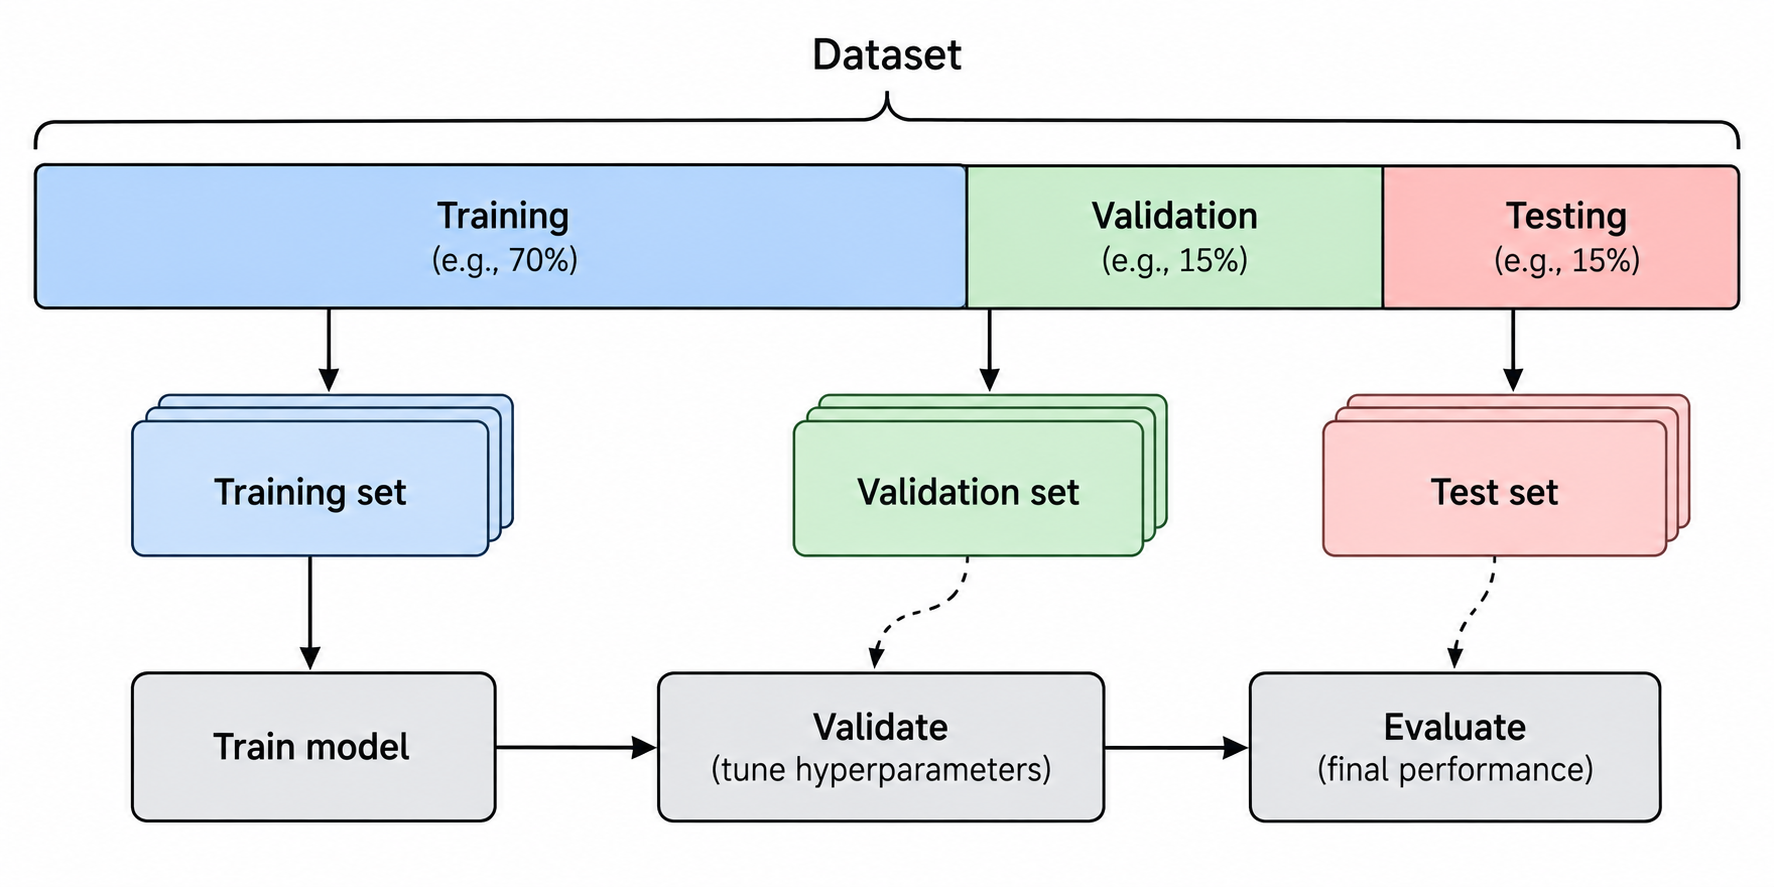
\includegraphics[height=3.3cm]{figures/dataset_split.png}}

\vspace{4pt}
\begin{itemize}
\small
\item \textbf{Training set}: fit the parameters $\bs{w}$ of each
  candidate model.
\item \textbf{Validation set}: held out from training, used to compare
  candidates and pick the best one.
\item \textbf{Test set}: held out until the very end, used
  \emph{once} for an unbiased estimate of performance on new data.
\end{itemize}

\end{frame}
%%%%%%%%%%%%%%%%%%%%%%%%%%%%%%%%%%%%%%%%%%%%%%%%%%%%%%%%%%%%%%%%%%%%%%
\begin{frame}[fragile]
\frametitle{Model selection: avoiding biased estimates}

\vfill
\begin{itemize}
\item[$\Rightarrow$] Never choose a model using test-set performance;
  that would bias the estimate of how well it generalises.
\vspace{10pt}
\item[$\Rightarrow$] Never \emph{test} on the training set either;
  training error is optimistically biased and does not reflect
  performance on new data.
\end{itemize}
\vfill

\end{frame}
%%%%%%%%%%%%%%%%%%%%%%%%%%%%%%%%%%%%%%%%%%%%%%%%%%%%%%%%%%%%%%%%%%%%%%
\begin{frame}[fragile]
\frametitle{Cross-validation}

\begin{columns}[T]
\begin{column}{0.45\textwidth}
\centerline{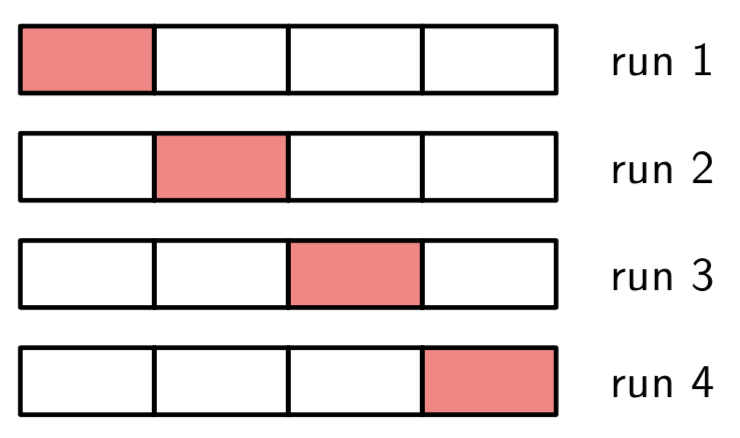
\includegraphics[width=\textwidth]{figures/prml_fig1_18.png}}

\vspace{4pt}
{\scriptsize Bishop, \emph{PRML} (2006), Fig.\ 1.18: 4-fold
cross-validation, in each of the 4 runs, one block (red) is held out
for validation and the rest (white) used for training.}
\end{column}
\begin{column}{0.52\textwidth}
\begin{itemize}
\item Problem: a fixed validation split wastes data that could
  otherwise be used for training, costly when labelled data is
  scarce.
\item \textbf{$S$-fold cross-validation}: partition the data into $S$
  groups. In turn, train on $S{-}1$ groups and validate on the
  remaining one; average performance over the $S$ runs.
\item Extreme case $S{=}N$: \textbf{leave-one-out} cross-validation.
\end{itemize}
\end{column}
\end{columns}

\vspace{6pt}
\begin{itemize}
\item[$\Rightarrow$] Cost: training must be repeated $S$ times; fine
  for cheap models, expensive for large ones (e.g.\ deep networks).
\end{itemize}

\end{frame}
%%%%%%%%%%%%%%%%%%%%%%%%%%%%%%%%%%%%%%%%%%%%%%%%%%%%%%%%%%%%%%%%%%%%%%
\begin{frame}[fragile]
\frametitle{Today: supervised learning, regression}

\begin{itemize}
\item Within supervised learning, the target $t$ can be:
  \begin{itemize}
  \item continuous $\Rightarrow$ \textbf{regression} (e.g.\ house price from
    features, the price-forecasting example above).
  \item discrete (a class label) $\Rightarrow$ \textbf{classification}
    (e.g.\ spam or not, dog or bagel); next lecture.
  \end{itemize}
\end{itemize}

\begin{itemize}
\item[$\Rightarrow$] \textbf{Today}: regression, curve fitting and least
  squares. Classification, and more on regression, follow next lecture.
\end{itemize}

\end{frame}
%%%%%%%%%%%%%%%%%%%%%%%%%%%%%%%%%%%%%%%%%%%%%%%%%%%%%%%%%%%%%%%%%%%%%%
\begin{frame}[fragile]
\frametitle{Motivating example: polynomial curve fitting}

\begin{columns}[T]
\begin{column}{0.4\textwidth}
\centerline{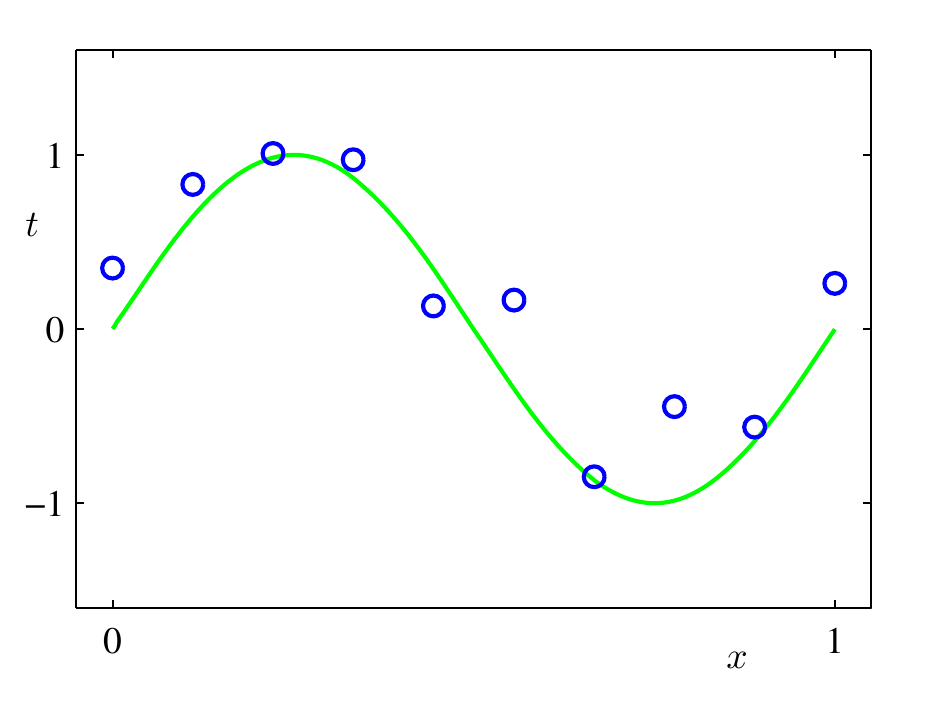
\includegraphics[width=\textwidth]{figures/prml_fig1_2.png}}

\vspace{4pt}
{\scriptsize Bishop, \emph{Pattern Recognition and Machine Learning}
(2006), Fig.\ 1.2: $N{=}10$ points (blue) sampled from $\sin(2\pi x)$
(green) plus random noise.}
\end{column}
\begin{column}{0.57\textwidth}
\begin{itemize}
\item Training set: $N$ observations of an input $x$, together with a
  target $t$: $\{(x_n,t_n)\}_{n=1}^N$.
\item For our running example, take $x$ and $t$ to be \textbf{scalars}
  (1D), as in the plot on the left, where $t_n$ is generated from
  $\sin(2\pi x_n)$ plus random noise.
\item Goal: predict $t$ for a \emph{new} $x$, i.e.\ learn a function
  $y(x,\bs{w})$.
\end{itemize}
\end{column}
\end{columns}

\vspace{6pt}
\begin{itemize}
\item Fit a polynomial of order $M$:
\[
y(x,\bs{w}) = w_0 + w_1 x + w_2 x^2 + \cdots + w_M x^M = \sum_{j=0}^{M} w_j x^j
\]
\item $\bs{w} = (w_0, w_1, \dots, w_M)^\top$ is the \textbf{weight
  vector}, the $M{+}1$ parameters we need to learn from the data.
\end{itemize}

\end{frame}
%%%%%%%%%%%%%%%%%%%%%%%%%%%%%%%%%%%%%%%%%%%%%%%%%%%%%%%%%%%%%%%%%%%%%%
\begin{frame}[fragile]
\frametitle{Linear basis function models}

\begin{itemize}
\item In general:
\[
y(x,\bs{w}) = \sum_{j=0}^{M-1} w_j\, \phi_j(x) = \bs{w}^\top \bs\phi(x)
\]
where $\phi_0(x) = 1$ (a bias term) and $\phi_1,\dots,\phi_{M-1}$ are fixed
\textbf{basis functions}.
\end{itemize}

\begin{itemize}
\item Common choices: polynomials ($\phi_j(x)=x^j$), Gaussians
  $\phi_j(x) = \exp\{-(x-\mu_j)^2/2s^2\}$, sigmoidal
  $\phi_j(x) = \sigma\bigl((x-\mu_j)/s\bigr)$.
\item[$\Rightarrow$] \textbf{Linear model} means linear in $\bs{w}$, \emph{not}
  linear in $x$ 
% \item A neural network (L04) relaxes exactly this: it \emph{learns} the
  % basis functions from data, instead of fixing them by hand.
\end{itemize}

\end{frame}
%%%%%%%%%%%%%%%%%%%%%%%%%%%%%%%%%%%%%%%%%%%%%%%%%%%%%%%%%%%%%%%%%%%%%%
\begin{frame}[fragile]
\frametitle{Least squares}

\begin{itemize}
\item Measure how well $y(x,\bs{w})$ fits the data with the
  \textbf{sum-of-squares loss function}:
\[
L_D(\bs{w}) = \frac{1}{2}\sum_{n=1}^{N} \bigl\{t_n - y(x_n,\bs{w})\bigr\}^2
\]
\item \textbf{Least squares}: choose $\bs{w}$ to minimise $L_D(\bs{w})$.
\end{itemize}

\begin{columns}[T]
\begin{column}{0.45\textwidth}
\centerline{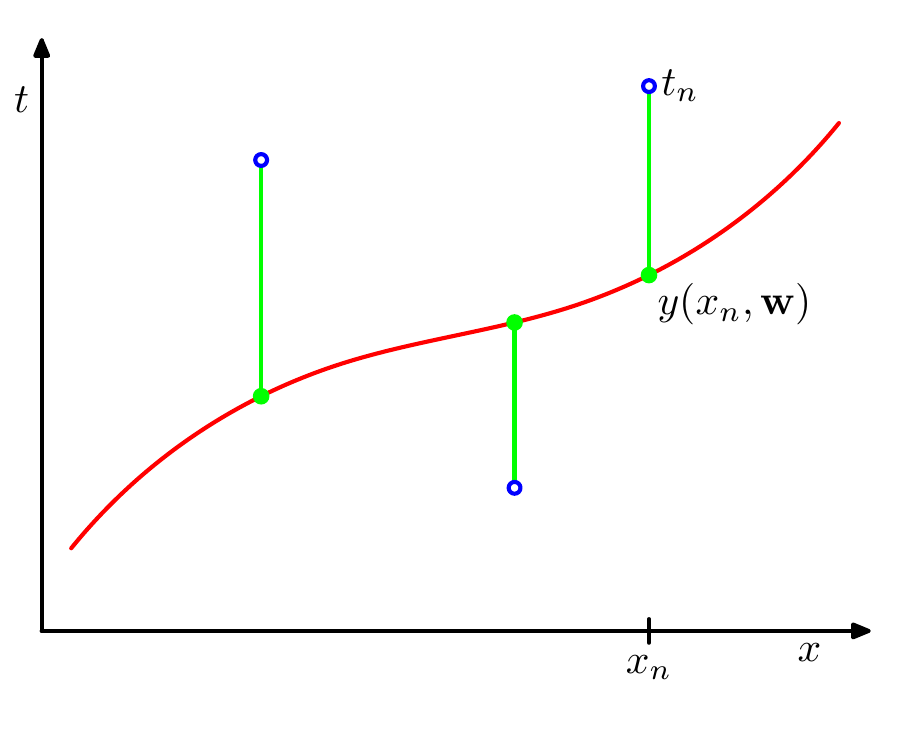
\includegraphics[width=\textwidth]{figures/prml_fig1_3.png}}

\vspace{2pt}
{\scriptsize Bishop, \emph{PRML} (2006), Fig.\ 1.3: each green bar is
one displacement $\{t_n - y(x_n,\bs{w})\}$, squared and summed to
give $L_D(\bs{w})$.}
\end{column}
\begin{column}{0.52\textwidth}
\begin{itemize}
\item Why squared error? Simple to optimise (differentiable, convex in
  $\bs{w}$), and, as we'll see shortly, it falls out naturally once we
  assume \textbf{Gaussian noise}.
\item[$\Rightarrow$] Because $y$ is linear in $\bs{w}$, $L_D$ is a
  \emph{quadratic} function of $\bs{w}$; it has a unique minimum,
  solvable in closed form.
\end{itemize}
\end{column}
\end{columns}

\end{frame}
%%%%%%%%%%%%%%%%%%%%%%%%%%%%%%%%%%%%%%%%%%%%%%%%%%%%%%%%%%%%%%%%%%%%%%
\begin{frame}[fragile]
\frametitle{Solving least squares: the design matrix}

\begin{itemize}
\item Stack the data: design matrix $\Phi \in \mathbb{R}^{N\times M}$ with
  $\Phi_{nj} = \phi_j(x_n)$, target vector $\bs{t} = (t_1,\dots,t_N)^\top$.
  Then $L_D(\bs{w}) = \frac12\|\bs{t}-\Phi\bs{w}\|^2$.
\end{itemize}

\centerline{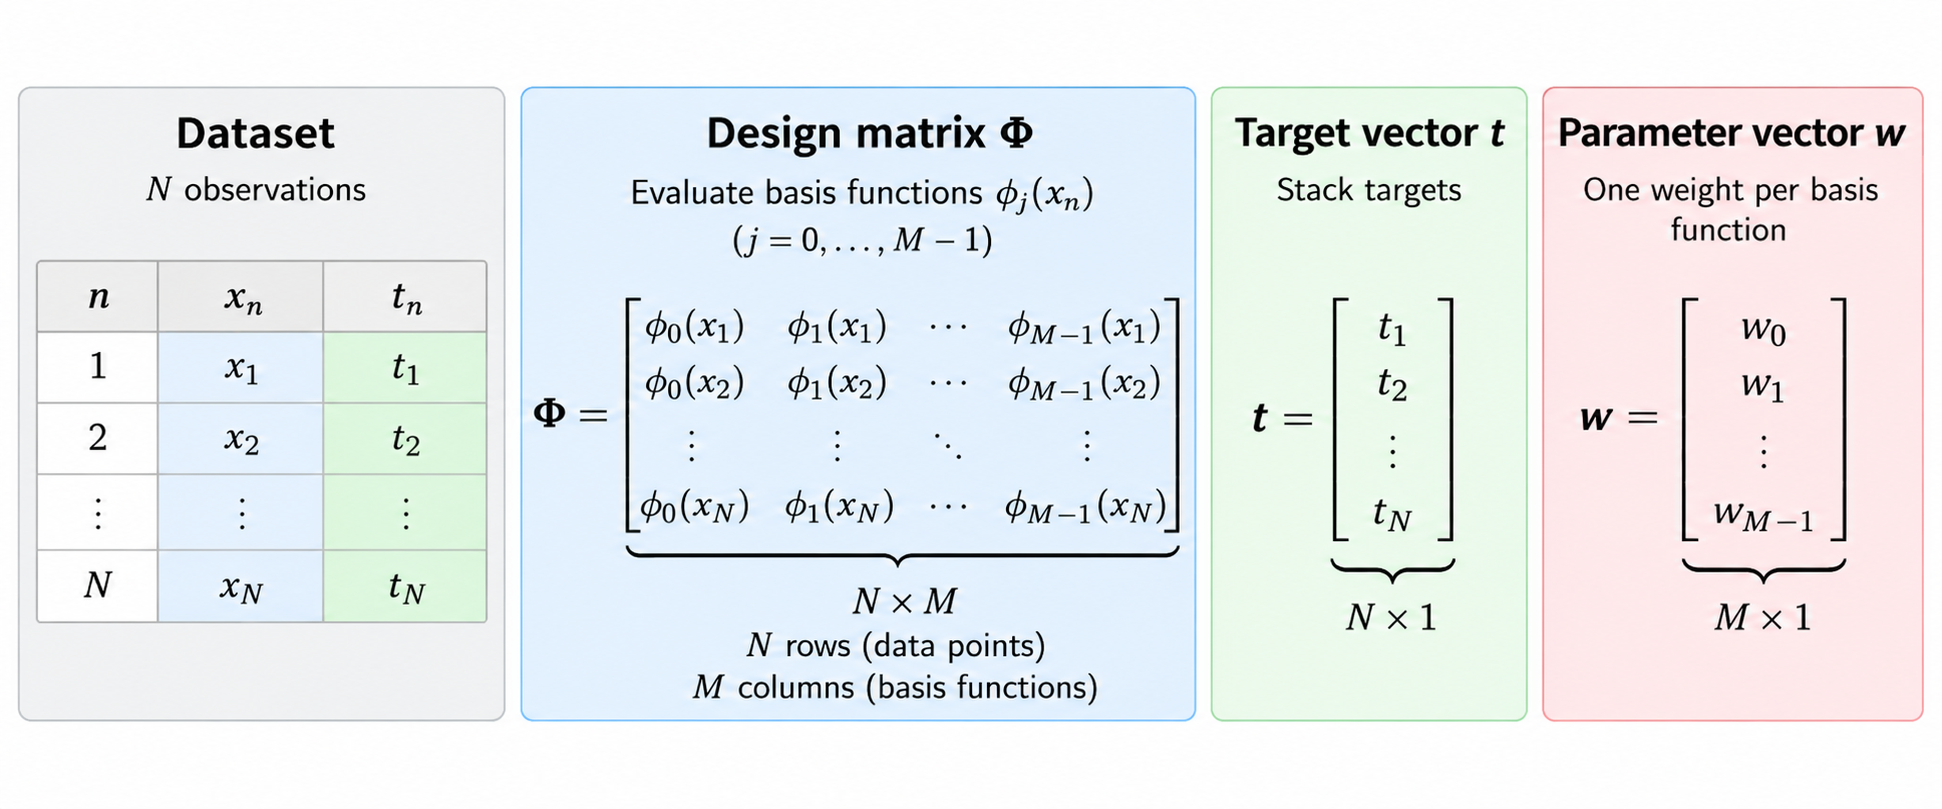
\includegraphics[width=0.95\textwidth]{figures/design_matrix.png}}

\end{frame}
%%%%%%%%%%%%%%%%%%%%%%%%%%%%%%%%%%%%%%%%%%%%%%%%%%%%%%%%%%%%%%%%%%%%%%
\begin{frame}[fragile]
\frametitle{Solving least squares: the normal equations}

\begin{itemize}
\item Recall $L_D(\bs{w}) = \frac12\|\bs{t}-\Phi\bs{w}\|^2$. Differentiating
  w.r.t.\ $\bs{w}$:
\[
\nabla_{\bs{w}} L_D(\bs{w}) = \Phi^\top\Phi\,\bs{w} - \Phi^\top\bs{t}
\]
\item Setting $\nabla_{\bs{w}} L_D(\bs{w}) = 0$ gives the \textbf{normal
  equations}:
\[
\Phi^\top \Phi\, \bs{w} = \Phi^\top \bs{t}
\]
\item Solution (the \textbf{least-squares}, or maximum-likelihood, estimate):
\[
\bs{w}_{\mathrm{ML}} = \bigl(\Phi^\top \Phi\bigr)^{-1} \Phi^\top \bs{t} =
\Phi^\dagger \bs{t}
\]
where $\Phi^\dagger$ is the (Moore-Penrose) \textbf{pseudo-inverse} of
$\Phi$.
\end{itemize}

% \begin{itemize}
% \item[$\Rightarrow$] One matrix computation gives the optimal $\bs{w}$
%   directly, no iterative search needed (though $\Phi^\top\Phi$ can be
%   ill-conditioned; more on numerical fixes when we meet regularization).
% \end{itemize}

\vspace{6pt}
{\scriptsize See Bishop, \emph{PRML} (2006), Section 3.1.1, for the full
derivation.}

\end{frame}
%%%%%%%%%%%%%%%%%%%%%%%%%%%%%%%%%%%%%%%%%%%%%%%%%%%%%%%%%%%%%%%%%%%%%%
\begin{frame}[fragile]
\frametitle{Try it: least squares by hand}

\begin{example}
Fit a straight line $y(x,\bs{w}) = w_0 + w_1 x$ (i.e.\ basis functions
$\phi_0(x){=}1$, $\phi_1(x){=}x$, so $M{=}2$) to the data:
\begin{center}
\begin{tabular}{c|c|c|c|c}
$x_n$ & $-1$ & $0$ & $1$ & $2$\\ \hline
$t_n$ & $0$ & $1$ & $3$ & $9$
\end{tabular}
\end{center}
\end{example}

\vspace{6pt}
\begin{itemize}
\item Before we go through it together: write down $\bs{t}$ and $\Phi$
  for this data, then use
  $\bs{w}_{\mathrm{ML}} = (\Phi^\top \Phi)^{-1} \Phi^\top \bs{t}$ to find
  $w_0$ and $w_1$.
\item[$\Rightarrow$] Try it on paper -- we'll work through the steps on
  the next slide.
\end{itemize}

\end{frame}
%%%%%%%%%%%%%%%%%%%%%%%%%%%%%%%%%%%%%%%%%%%%%%%%%%%%%%%%%%%%%%%%%%%%%%
\begin{frame}[fragile]
\frametitle{Least squares: a worked example}

\small
\begin{example}
Fit a straight line $y(x,\bs{w}) = w_0 + w_1 x$ (i.e.\ basis functions
$\phi_0(x){=}1$, $\phi_1(x){=}x$, so $M{=}2$) to the data:
\begin{center}
\begin{tabular}{c|c|c|c|c}
$x_n$ & $-1$ & $0$ & $1$ & $2$\\ \hline
$t_n$ & $0$ & $1$ & $3$ & $9$
\end{tabular}
\end{center}
\end{example}

\uncover<2->{$\bs{t} = \begin{bmatrix} 0\\ 1\\ 3\\ 9 \end{bmatrix}$}
\hspace{6pt}
\uncover<3->{$\Phi = \begin{bmatrix} 1 &-1\\ 1&0\\ 1 &1\\ 1 &2 \end{bmatrix}$}
\hspace{6pt}
\uncover<4->{$\Phi^\top \Phi = \begin{bmatrix} 1 &1 &1 &1\\ -1 &0 &1 &2
  \end{bmatrix} \begin{bmatrix} 1 &-1\\ 1&0\\ 1 &1\\ 1 &2 \end{bmatrix} =
  \begin{bmatrix} 4 &2\\ 2 &6\end{bmatrix}$}

\uncover<5->{$\bs{w}_{\mathrm{ML}} = (\Phi^\top \Phi)^{-1} \Phi^\top \bs{t}$}
\uncover<6->{$= \dfrac{1}{20}\begin{bmatrix} 6 &-2\\ -2 &4 \end{bmatrix}$}
\uncover<7->{$\begin{bmatrix} 1 &1 &1 &1\\ -1 &0 &1 &2 \end{bmatrix}$}
\uncover<8->{$\begin{bmatrix} 0\\ 1\\ 3\\ 9 \end{bmatrix}$}
\uncover<9->{$= \begin{bmatrix} 1.8\\ 2.9 \end{bmatrix}$}

\uncover<10->{$\Rightarrow\ y(x,\bs{w}_{\mathrm{ML}}) = 1.8 + 2.9\,x$}

\vspace{6pt}
{\scriptsize Example adapted from the \emph{Machine Learning} unit
(COMS30035).}

\end{frame}
%%%%%%%%%%%%%%%%%%%%%%%%%%%%%%%%%%%%%%%%%%%%%%%%%%%%%%%%%%%%%%%%%%%%%%
\begin{frame}[fragile]
\frametitle{How to evaluate a regression task: evaluation metrics}

\small
\begin{itemize}
\item \textbf{Mean squared error (MSE)}:
\[
\mathrm{MSE} = \frac{1}{N}\sum_{n=1}^N \bigl\{t_n - y(x_n,\bs{w})\bigr\}^2
\]
  \begin{itemize}
  \item Same shape as $L_D(\bs{w})$ (up to the $\frac12$ and the
    averaging); squaring means large errors are penalised heavily.
  \end{itemize}
\item \textbf{Root mean squared error (RMSE)}: $\sqrt{\mathrm{MSE}}$,
  back in the same units as $t$ (this is $E_{\mathrm{RMS}}$ from
  Fig.\ 1.5).
\item \textbf{Mean absolute error (MAE)}:  More robust to outliers than MSE/RMSE, since errors are not
    squared.
\[
\mathrm{MAE} = \frac{1}{N}\sum_{n=1}^N \bigl|t_n - y(x_n,\bs{w})\bigr|
\]
\item \textbf{$R^2$ (coefficient of determination)}: the fraction of
  the variance in $t$ explained by the model; $R^2{=}1$ is a perfect
  fit, $R^2{=}0$ is no better than always predicting the mean of $t$.
\end{itemize}

% \begin{itemize}
% \item[$\Rightarrow$] Always compute these metrics on held-out
%   (validation or test) data, not on the training set used to fit
%   $\bs{w}$.
% \end{itemize}

\end{frame}
%%%%%%%%%%%%%%%%%%%%%%%%%%%%%%%%%%%%%%%%%%%%%%%%%%%%%%%%%%%%%%%%%%%%%%
\begin{frame}[fragile]
\frametitle{Summary}

\vfill
\begin{itemize}
\item \textbf{Categories of ML}: supervised, unsupervised, reinforcement,
  self-/semi-supervised
\vspace{6pt}
\item \textbf{Model selection}: train / validation / test split;
  cross-validation; never touch the test set until the end
\vspace{6pt}
\item \textbf{Regression}: linear-in-$\bs{w}$ models,
  $y(x,\bs{w}) = \bs{w}^\top\bs\phi(x)$
\vspace{6pt}
\item \textbf{Least squares}: minimise
  $L_D(\bs{w}) = \frac12\|\bs{t}-\Phi\bs{w}\|^2 \Rightarrow
  \bs{w}_{\mathrm{ML}} = \Phi^\dagger \bs{t}$
\vspace{6pt}
\item \textbf{Evaluation}: MSE/RMSE/MAE and $R^2$, always on held-out
  data
\vspace{6pt}
\item[$\Rightarrow$] Next lecture: the probabilistic view of least
  squares, stochastic gradient descent, regularization, and
  classification (logistic regression).
\end{itemize}
\vfill

\end{frame}
%%%%%%%%%%%%%%%%%%%%%%%%%%%%%%%%%%%%%%%%%%%%%%%%%%%%%%%%%%%%%%%%%%%%%%
\begin{titledslide}{Reading}

  \begin{itemize}
  \item Bishop, C.\,M., \emph{Pattern Recognition and Machine Learning}
    (2006).
    \href{https://www.microsoft.com/en-us/research/uploads/prod/2006/01/Bishop-Pattern-Recognition-and-Machine-Learning-2006.pdf}{Free
      online}.
  \item Today's material: Chapter 1 (\S1.1, \S1.3), Chapter 3 (\S3.1).
  % \item We follow Bishop's notation throughout, inputs $x$, targets $t$,
    % basis functions $\bs\phi(x)$, weights $\bs{w}$.
  \end{itemize}

\end{titledslide}
%%%%%%%%%%%%%%%%%%%%%%%%%%%%%%%%%%%%%%%%%%%%%%%%%%%%%%%%%%%%%%%%%%%%%%
\end{document}
